\documentclass[11pt, a4paper]{article}
\usepackage{amsmath, amsfonts, dsfont, booktabs, graphicx, natbib, a4wide, times, microtype, hyperref}
\newcommand{\E}{\ensuremath{{\mathbb E}}} % expected value
\def\func#1{\mathop{\rm #1}}
\begin{document}
\title{Solution to Exercise 3}
\author{Simon A.\ Broda}
\date{}
\maketitle
\begin{enumerate}
\item
\begin{enumerate}
\item We clearly see that unless $|\phi_1|$ approaches 1, the process is stationary; the time series plot looks mean-reverting, and the sample autocorrelations decay exponentially as they should. We also see that $\bar y$ is close to $\E[Y_t]=\alpha/(1-\phi_1)$, and that $s^2_y$ is close to $\func{var}[Y_t]=\sigma^2/(1-\phi_1^2)$.
\item If $\phi_1=1$, we have a random walk, and $\alpha$ becomes the drift: $\E[Y_t]=Y_0+\alpha\cdot t$.
\item The correlograms of the AR(1), MA(1), and ARMA(1, 1) look respectively as follows.
\begin{center}
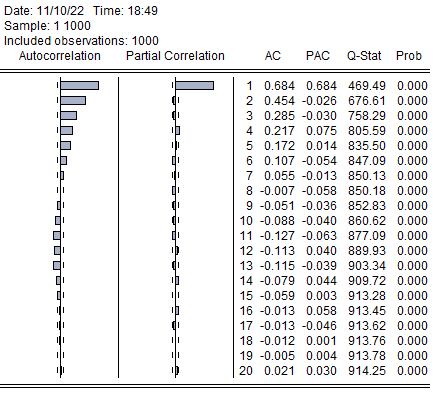
\includegraphics[width=.6\textwidth]{ar1_acf}
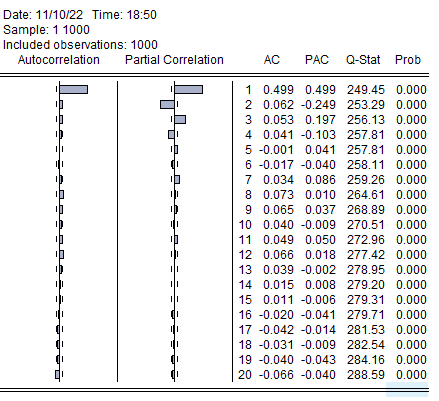
\includegraphics[width=.6\textwidth]{ma1_acf}
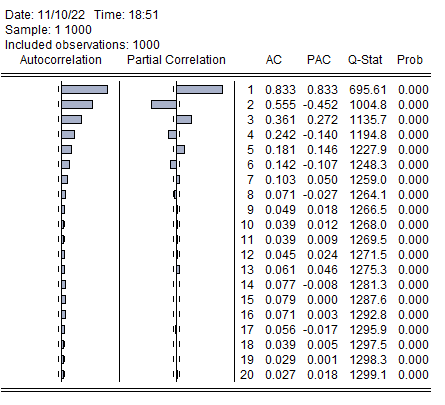
\includegraphics[width=.6\textwidth]{arma11_acf}
\end{center}
For the AR(1), we see that the SACF decays geometrically, while the SPACF drops to zero (more or less) after 1 lag. For the MA(1), we see that the picture is reversed (the fact that the sign of the SPACF alternates does not play a role, as long as its absolute value decays geometrically). For the ARMA(1, 1), both SACF and SPACF decay geometrically, so it's impossible to determine the order of an ARMA($p$, $q$) process (here, $p=1$ and $q=1$) from the correlogram.
\end{enumerate}
\item
\begin{enumerate}
\item The correlogram looks as shown below.
\begin{center}
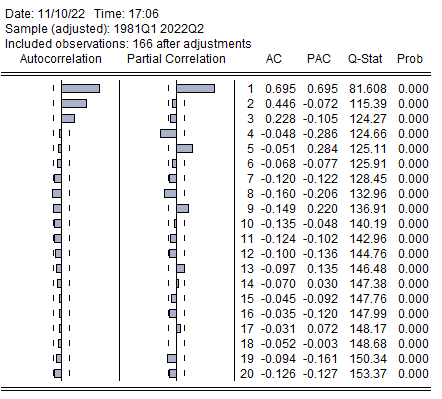
\includegraphics[width=.6\textwidth]{corr_gdpg}
\end{center}
Geometrically decaying ACF, PACF drops to zero after one lag, even though some later values are significant. Still, a simple AR(1) might suffice. We can estimate it by entering \verb.gdp_growth c ar(1). under \texttt{Quick$\rightarrow$ Estimate Equation\ldots}. The result is
\begin{center}
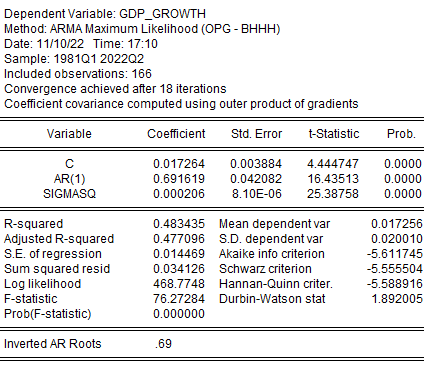
\includegraphics[width=.6\textwidth]{ar1_gdpg}
\end{center}
Everything is significant, and the estimated model is stationary (AR coefficient is less than 1 in absolute value). The residual correlogram (under \texttt{View$\rightarrow$Residual\linebreak Diagnostics\ldots} looks like this:
\begin{center}
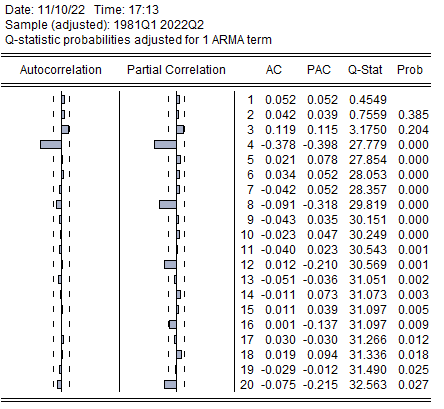
\includegraphics[width=.6\textwidth]{corr_ar1_gdpg}
\end{center}
The ACF and PACF at lag 4 are both significant. It's not obvious which model to use for this. One idea is to use an ARMA(1, 4), which we can estimate by entering \verb.gdp_growth c ar(1) ma(1 to 4). in the estimation window, resulting in the estimation output and residual correlogram below.
\begin{center}
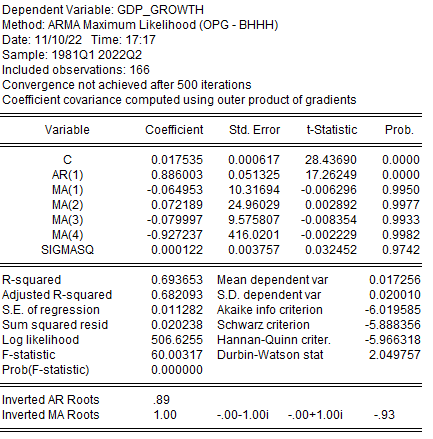
\includegraphics[width=.6\textwidth]{arma14_gdpg}
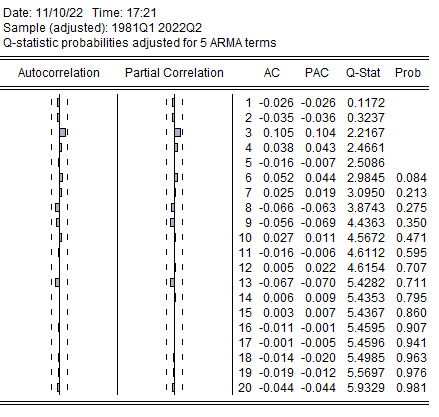
\includegraphics[width=.6\textwidth]{corr_arma14_gdpg}
\end{center}
The residual correlogram looks fine now, but note that all the MA coefficients are insignificant. Maybe we can get away with dropping the first 3, leading to the \emph{subset AR model}
\[
Y_t= \alpha+\phi_1 Y_{t-1}+ U_t + \theta_4 U_{t-4}.
\]
This can be estimated by entering \verb.gdp_growth c ar(1) ma(4). in the estimation window. The results are shown below.
\begin{center}
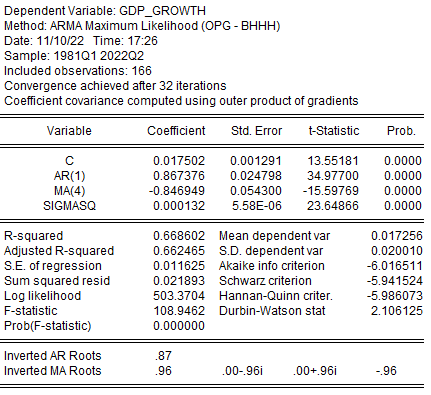
\includegraphics[width=.6\textwidth]{arma14subset_gdpg}
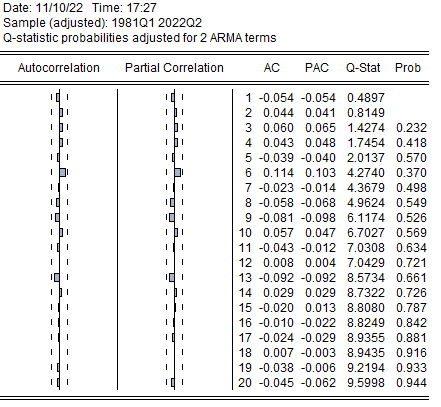
\includegraphics[width=.6\textwidth]{corr_arma14subset_gdpg}
\end{center}
The correlogram still looks fine, and all coefficients are now significant. The subset model has a smaller BIC (-5.94 vs.\ -5.89), so is preferred (better tradeoff between fit and parsimony). The AIC seems to prefer the larger model; this is typical.

Instead of the above manual procedure, we can automate the procedure of finding the model by using \href{https://www.eviews.com/help/helpintro.html#page/content%2Fseriescmd-autoarma.html}{autoarma}: just paste

\begin{verbatim}freeze(armatable) gdp_growth.autoarma(diff=0
, select=sic, maxar=4, maxma=4, atable) forec c
\end{verbatim}
into the estimation window (all on one line).
This produces the table below.
\begin{center}
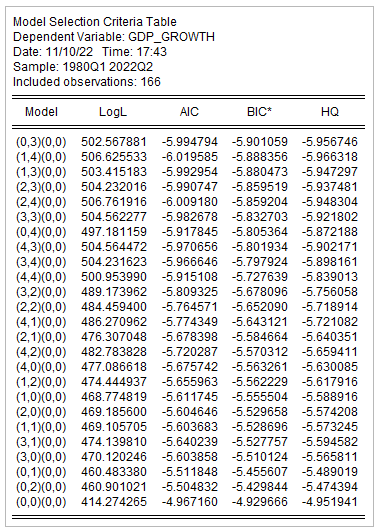
\includegraphics[width=.6\textwidth]{autoarma}
\end{center}
We see that the BIC selects a MA(3) model\footnote{The AIC selects an ARMA(1, 4)}, but it has a higher BIC than our subset model, because \verb.autoarma. doesn't consider subset models. Estimating this model via
\begin{verbatim}
gdp_growth c ma(1 to 3)
\end{verbatim}
results in the output below.
\begin{center}
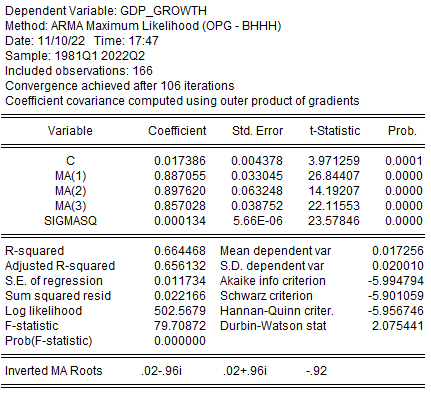
\includegraphics[width=.6\textwidth]{ma3_gdpg}
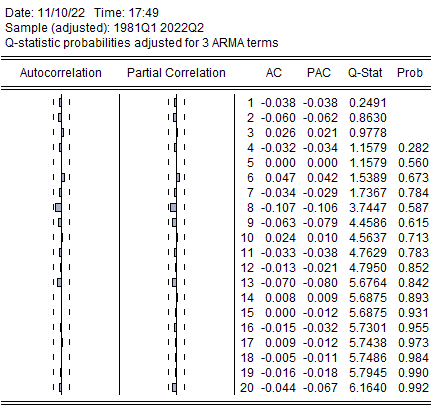
\includegraphics[width=.6\textwidth]{corr_ma3_gdpg}
\end{center}
This looks fine too. I prefer to stick with our subset model, because it has a lower BIC.
\item The estimated parameter \texttt{c} in EViews corresponds to $c=\E[Y_t]=\alpha/(1-\phi_1)$, so we have $\hat{\alpha}=\hat{c}(1-\hat{\phi}_1)=0.017502\cdot(1-0.867376)=0.002321$.  Thus, our final model is
\[
Y_t= 0.002321+ 0.867376 Y_{t-1}+ U_t -0.846949 U_{t-4}.
\]

The manual forecast for 2022Q3 is therefore
\begin{align*}
\widehat{y}_{t+1}&= 0.002321+0.867376\cdot 0.024037-0.846949\cdot0.001429\\
&=0.021960.
\end{align*}
 The value for $y_{2022Q2}$, 0.024037, can be obtained from the spreadsheet view.
The value 0.001429 corresponds to $\hat{u}_{2021Q3}$. To find it, go to the estimation output, click on \texttt{Proc$\rightarrow$Make Residual Series...}, and open the resulting series in spreadsheet view.

The manual forecast for 2022Q4 can be constructed analogously. It requires $y_{2022Q3}$, which we replace with our forecast from the previous question. Hence
\begin{align*}
\widehat{y}_{t+2}&= 0.002321+0.867376\cdot 0.021960-0.846949\cdot(-0.003883)\\
&=0.024657,
\end{align*}
where $-0.003883=\hat{u}_{2021Q4}$.
The same forecasts can be obtained using EViews. First, inside the workfile pane on the left, go to \texttt{Proc}$\rightarrow$\linebreak\texttt{Structure / Resize Current Page\ldots}, and resize the file so that it includes 2022Q3 and 2022Q4. Next, in the pane with the estimation output, click on \texttt{Forecast}. Keep the default of a dynamic forecast, and set the forecast sample to 2022Q3:2022Q4. Your forecast will be saved as a new series \verb.gdp_growthf. You can open it in spreadsheet view and confirm that the forecasts are the same as those obtained above,
\end{enumerate}
\item
\begin{enumerate}
\item By repeatedly plugging in,
\begin{eqnarray*}
Y_t&=&\alpha+Y_{t-1}+U_t\\
   &=&\alpha+(\alpha +Y_{t-2}+U_{t-1})+U_t\\
  &\vdots&\\
&=&Y_0+\alpha\cdot t+\sum_{s=1}^t U_s,
\end{eqnarray*}
so that
\[
\E[Y_t]=Y_0+ \alpha\cdot t,
\]
because white noise has expectation zero. The derivation of the variance is the same as for the case without drift from last week and thus omitted here.
\item The previous question shows that the random walk with drift is not stationary, because its mean and variance change over time. For it to be I(1), its first difference $\Delta Y_t$ should be stationary.
We immediately se that $\Delta Y_t=Y_t-Y_{t-1}=(\alpha+Y_{t-1}+U_t)-Y_{t-1}=\alpha + U_t$. This is just white noise plus a constant, which is stationary.
\item
Since $\{U_t\}$ is white noise, $U_t$  is uncorrelated with $Y_{t-1}$, so
\begin{align*}
\mathrm{var}(Y_t) &= \func{var}\left(\alpha+\phi_1Y_{t-1}+U_{t}\right)\\
&= \phi_1^2 \mathrm{var}(Y_{t-1}) + \mathrm{var}(U_t) + 2
\phi_1 \mathrm{cov}(Y_{t-1},U_{t})
&= \phi_1^2 \mathrm{var}(Y_{t}) +
\sigma^2,
\end{align*}
where the final equality holds because $Y_t$ is stationary, which implies that $\func{var}(Y_t)=\func{var}(Y_{t-1})$. Thus, if and only if $|\phi_1 |<1$,
\begin{equation*}
\mathrm{var}(Y_t) = \frac{\sigma^2}{1-\phi_1^2}.
\end{equation*}
Note that $\mathrm{var}(Y_t) > \mathrm{var}(Y_{t-1})$ if $|\phi_1 |\ge 1$, i.e., the variance grows without bounds in that case.
\item For the MA(1) process
\begin{equation*}
Y_t=\alpha + U_t + \theta_1 U_{t-1},
\end{equation*}
we have that
\begin{align*}
\E[Y_t]&=\E[\alpha + U_t + \theta_1 U_{t-1}]\\
&=\alpha + \E[U_t] + \theta_1 \E[U_{t-1}]\\
&=\alpha.
\end{align*}
For the variance,
\begin{align*}
\gamma_0&=\func{var}(Y_t)=\func{var}(\alpha + U_t + \theta_1 U_{t-1})\\
&=\func{var}(U_t + \theta_1 U_{t-1})\\
&=\func{var}(U_t) + \theta_1^2\func{var}( U_{t-1})+2\theta_1\func{cov}(U_t, U_{t-1})\\
&=\sigma^2+\theta_1^2\sigma^2+0\\
&=\sigma^2(1+\theta_1^2).
\end{align*}
For the first autocovariance,
\begin{align*}
\gamma_1&=\func{cov}(Y_t, Y_{t-1})\\
&=\func{cov}(\alpha + U_t + \theta_1 U_{t-1}, \alpha + U_{t-1} + \theta_1 U_{t-2})\tag{$\dagger$}\label{ma}\\
&=\func{cov}(\theta_1 U_{t-1},U_{t-1})\\
\intertext{because white noise is uncorrelated. Hence}
\gamma_1&=\theta_1\func{cov}( U_{t-1},U_{t-1})\\
&=\theta_1\func{var}(U_{t-1})\\
&=\theta_1\sigma^2.
\end{align*}
Higher order autocorrelations will be zero, because there will no common $U_t$ terms in \eqref{ma}.
Plugging these into the definition of the ACF, we have
\[
\tau_1=\frac{\gamma_1}{\gamma_0}=\frac{\theta_1\sigma^2}{\sigma^2(1+\theta_1^2)}=\frac{\theta_1}{1+\theta_1^2}.
\]


\item \textbf{Optional}:
The ACF is obtained by repeatedly
substituting $Y_{t-i} = \phi_1 Y_{t-i-1} + \alpha + U_{t-i}$:
\begin{eqnarray}
Y_t &=&\phi_1 Y_{t-1}+ \alpha + U_t  \notag \\
&=&\phi_1 ^2Y_{t-2} + \phi_1 (\alpha + U_{t-1}) + \alpha + U_t  \notag \\
&=&\phi_1 ^3 Y_{t-3}+ \phi_1 ^2 (\alpha + U_{t-2} )+ \phi_1 (\alpha + U_{t-1})+
\alpha + U_t  \notag \\
&\vdots &  \notag \\
&=&\phi_1 ^k Y_{t-k}+\sum_{i=0}^{k-1}\phi_1 ^i \alpha + \sum_{i=0}^{k-1}\phi_1
^i U_{t-i}.  \label{subst}
\end{eqnarray}

Therefore,
\begin{align*}
\gamma_k &= \mathrm{cov}(Y_t,Y_{t-k}) = \phi_1 ^k \mathrm{cov}%
(Y_{t-k},Y_{t-k}) + \sum_{i=0}^{k-1}\phi_1 ^i \mathrm{cov}(U_{t-i},Y_{t-k})\\
&= \phi_1 ^k \mathrm{var}(Y_{t-k}),
\end{align*}
so that
\begin{equation*}
\tau_k = \frac{\gamma_k}{\gamma_0} = \phi_1 ^k.
\end{equation*}

\end{enumerate}
\end{enumerate}
\end{document} 